\iftrue
\section{IMPLEMENTATION}
\label{ch:implementation}

%於前一章節（\S \ref{ch:design}）中已經闡述了選項分析、選項參數探索、多參數 forkserver 的基本原理，本章節會進一步說明選項感知模糊測試原型 KOFTA 的實作細節與挑戰。
%The previous section (\S \ref{ch:design}) has already explained the basic principles of option analysis, optional argument exploration, and multi-argument forkserver. 
This section will further explain the implementation details and challenges of the option-aware fuzzing prototype.
\fi

\iftrue

\subsection{Option Analysis} %選項分析

%KOFTA 首先透過靜態分析從原始碼中提取選項，接著透過動態分析過濾出合法的選項組合，同時利用污染源推論評估選項的選項參數必要性。
%實作上採用編譯階段的LLVM Pass達成。
In practice, this is achieved using LLVM Pass during the compilation phase.

\subsubsection{LLVM Pass}
\label{subsec:llvm-pass}

%AFL 紀錄分支覆蓋率的插樁模式有兩種：從組合語言層級分析，尋找特定的標籤或是指令，直接插入紀錄覆蓋率的程式碼片段；或是使用 LLVM 框架，從相對抽象的語法樹分析，在目標處新增紀錄覆蓋率的語法節點。
%使用 LLVM 框架的好處除了編譯時能夠對插樁後的語法樹進行優化以外，還可以有系統地分析目標程式原始碼。在 LLVM 框架中可以從模組、函式、基本區塊、指令等層級分析。例如分支覆蓋率就是從基本區塊分析、插樁；
%
%而支援KOFTA 靜態分析、動態分析和污染源推論的插樁皆是「指令」層級的分析。
The instrumentation that supports KOFTA static analysis, dynamic analysis, and taint inference is all at the "instruction" level.
%分析用的流程以 C++ 撰寫並稱為 LLVM Pass 。

%靜態分析時會找出所有「呼叫（call）」之對象為關鍵函式（如 \texttt{strcmp()}、 \texttt{getopt()}、 \texttt{getopt\_long()} 等）的指令，並提取呼叫時帶入的參數進行分析。對於呼叫 \texttt{strcmp()} 的指令，會分析其參數是否為一個在編譯階段確定的字串，若可以在編譯階段確定字串的內容則會檢查該字串是否以「\texttt{-}」開頭，提取可能的選項；對於呼叫 \texttt{getopt()}、 \texttt{getopt\_long()} 的指令，同樣會檢查其參數 \texttt{optstring}、\texttt{longopts} 是否可在編譯階段確定其值，若內容確定則從中提取可用的選項、對應的選項參數必要性。提取選項的同時，也會生成該關鍵函式對應的識別碼，並在該呼叫指令前增加新的語法節點，呼叫用於動態分析的 \texttt{\_\_kofta\_optana()}。

\subsubsection{Option File} %選項文件

%LLVM Pass在靜態分析找到的選項會紀錄至一份「選項文件」中（Listing \ref{lst:opttxt-example}），由同一個關鍵函式提取的選項會組成一個選項群組。每個選項群組的第一行會紀錄其識別碼、群組大小，接著一行紀錄一個選項，每行開頭為一個 \texttt{0} 至 \texttt{2} 的整數，分別代表選項參數必要性的「無」、「必要」、「非必要」，接著一個空白後是選項本身。選項文件會在測試時提供給 KOFTA 根據動態分析的結果產生合理的選項組合。
LLVM Pass records the options found during static analysis in an "option file". Options extracted by the same critical function are grouped together. The first line of each option group records its identifier and group size, followed by a single option on each line. Each line begins with an integer between \texttt{0} and \texttt{2}, representing the option's necessity as "none," "necessary," or "non-necessary," respectively, followed by a space and the option itself. The option file is provided to KOFTA during testing to generate appropriate option combinations based on the results of dynamic analysis.

\iffalse
%\begin{lstlisting}[float=h!, language=TeX, caption=選項文件範例, label=lst:opttxt-example]
\begin{lstlisting}[float=h!, language=TeX, caption=Option File, label=lst:opttxt-example]
23927 4
0 -C
0 -D
1 -t
0 -n
62376 3
0 -h
2 -d
0 -q
11514 3
1 -D
1 -H
0 -v
\end{lstlisting}
\fi

\subsubsection{Critical Function} %關鍵函式
\label{subsec:optana-key-funcs}

%靜態分析的關鍵函式除了 \texttt{strcmp()} 以外，還有幾個常用於字串匹配的函式也應納入考慮：\texttt{strcasecmp()}、\texttt{strncmp()}、\texttt{strncasecmp()}、\texttt{memcmp()}。此外，除了使用 \texttt{getopt()}、 \texttt{getopt\_long()} 解析命令列參數，許多專案會實做自己版本的解析函式。而這些函式所接受的參數往往與 GNU 的標準類似或是相同，因此 KOFTA 也將所有名稱包含「\texttt{getopt}」字串的函式皆當作關鍵函式，嘗試對其參數進行分析。
\texttt{strcmp()}, \texttt{memcmp()}, \texttt{getopt()}, and \texttt{getopt\_long()} are considered.

\subsubsection{Minimum Arguments} %基本參數數量限制

%初期的 KOFTA 會從不帶任何選項開始測試，直到動態分析回饋識別碼再從選項文件中尋找可用的選項。但是考慮以下目標程式（Listing \ref{lst:basic-argc-constraint}）中，由於最低參數數量的限制，不帶選項則無法觸發動態分析函式 \texttt{\_\_kofta\_optana()}。為了應對這種情況，在動態分析無法蒐集任何識別碼時 KOFTA 會產生一組虛設（dummy）選項：\texttt{--kofta k}，並持續增加虛設選項之組數直到通過最低基本參數數量限制、產生識別碼的回饋。
Continue to increase the number of dummy options until the minimum arguments limit is met and a feedback identification code is generated.

\iffalse
%\begin{lstlisting}[float=h!, caption=基本參數數量限制範例, label=lst:basic-argc-constraint]
\begin{lstlisting}[float=h!, caption={\footnotesize Limitation of the Numbers of Arguments}, label=lst:basic-argc-constraint]
int main(int argc, char** argv)
{
  if (argc < 4) exit(1);

  __kofta_optana(23927);
  while ((opt = getopt(argc, argv, "nt:")) != -1)
  {
    // ...
  }
}
\end{lstlisting}
\fi

\fi % \subsection{Option Analysis}

\iftrue

\subsection{Exploring Optional Arguments} %選項參數探索

%選項參數探索主要基於污染源推論，污染源推論所需的插樁與之前章節（\S \ref{subsec:llvm-pass}）的靜態分析一同由 LLVM Pass 完成。

%\subsubsection{Taint Sink} %污染終點

%污染源推論需要插樁的污染終點有三，一是「呼叫字串匹配函式」的指令，二是「比較（cmp）」指令，三是「switch」指令。對於呼叫字串匹配函式的指令，會分析其參數是否為一個在編譯階段確定的字串，若可以確定字串的內容則會檢查該字串是否以「\texttt{-}」開頭，因為污染源推論的目標是探索選項參數，所以對於以「\texttt{-}」開頭的字串會略過不處理，反之將該字串紀錄下來；對於比較指令，會檢查比較條件是否恰好有一個運算元是常數（constant）且該常數不為零，因為運算元皆為非常數的條件較難通過，皆為常數又沒有分析的必要，至於略過常數為零的比較條件是因為預設輸入的選項參數就是 \texttt{0} ，蒐集提示為 \texttt{0} 的回饋效果不大；對於 switch 指令則會蒐集所有目標（case）的值。LLVM Pass 會根據類別在污染終點前插樁：\texttt{\_\_kofta\_trace\_str()}、 \texttt{\_\_kofta\_trace\_cmp()}、  \texttt{\_\_kofta\_trace\_swt()}，在執行階段生成對應的鏈結串列、提示回饋。此處「字串匹配函式」與關鍵函式章節（\S \ref{subsec:optana-key-funcs}）中列舉的函式相同。

%\subsubsection{Boundary Analysis for Optional Argument} %選項參數邊界分析

%一個選項參數可能由多個「欄位」組成，考慮目標程式（Listing \ref{lst:multi-field-optarg-example}）中對於選項「\texttt{--paper}」的選項參數解析，污染終點有四個：「\texttt{strlen(arg) < 3}」、「\texttt{arg[2] != 'x'}」、「\texttt{paper->w < 30}」、「\texttt{paper->h < 50}」。選項「\texttt{--paper}」的選項參數由三個部份組成：整數（大於等於 \texttt{30}）、分割符（\texttt{x}）、整數（大於等於 \texttt{50}）。假設使用「\texttt{--paper kofta}」進行首次的測試，由於選項參數不合法，目標程式會在 Line 6 因為「\texttt{'f' != 'x'}」結束程式。接著逐一對選項參數的每一個位元組進行污染源推論，前兩組測試的選項參數為「\texttt{lofta}」、「\texttt{kpfta}」，不僅程式執行路徑與首次測試時完全相同，鏈結串列中的節點狀態也沒有改變；直到第三組測試「\texttt{kogta}」時，鏈結串列中「\texttt{arg[2] != 'x'}」比較條件的節點狀態發生了改變，比較從「\texttt{'f' != 'x'}」變成了「\texttt{'g' != 'x'}」，因此可以推論選項參數中的第三個位元組可能影響這個分支的結果，並知道有關的提示是「\texttt{x}」。根據提示 KOFTA 生成了「\texttt{--paper koxta}」進行測試並產生了新的執行路徑，並以新的路徑作為基準進行下一輪的污染源推論。

%此時「\texttt{atoi("koxta")}」與「\texttt{atoi("ta")}」的結果是 \texttt{0}，都會造成目標程式在 Line 12 結束。使用「\texttt{1oxta}」測試雖然執行路徑不變，但節點「\texttt{paper->w < 30}」的狀態從「\texttt{0 < 30}」變成了「\texttt{1 < 30}」，於是推論選項參數的第一個位元組與這個節點的分支有關，得到提示「\texttt{30}」後，使用「\texttt{--paper 30xta}」測試並產生新的執行路徑（避免了短路運算，產生「\texttt{paper->h < 50}」的節點）。以此類推，繼續使用污染源推論可以完整得到「\texttt{--paper 30x50}」的選項參數組合。

%\vfill
\iffalse
%\begin{lstlisting}[float=h!, caption=多欄位選項參數範例, label=lst:multi-field-optarg-example]
\begin{lstlisting}[float=h!, caption=Multi-Field Optional Arguments, label=lst:multi-field-optarg-example]
if (!strcmp(argv[i], "--paper"))
{
  char *arg = argv[i + 1];
  if (strlen(arg) < 3 || arg[2] != 'x')
  {
    exit(1);
  }
  paper->w = atoi(arg);
  paper->h = atoi(arg + 3);
  if (paper->w < 30 || paper->h < 50)
  {
    exit(1);
  }
}
\end{lstlisting}
\fi
%考慮以「\texttt{--paper 30xta}」為基準的污染源推論，不論測試選項參數為「\texttt{40xta}」或是「\texttt{31xta}」，都可以從相同的節點（\texttt{paper->w < 30}）得到相同的提示「\texttt{30}」，因此可以推論選項參數中的第一個位元組與第二個位元組應屬於同一個「欄位」。對於選項參數中連續且得到相同提示的位元組，會視為一個欄位並根據提示從該欄位的第一個位元組開始替換；換句話說，只會產生「\texttt{30xta}」而不會有「\texttt{330ta}」。

%然而實際情況是，所有的選項參數都是從虛設選項參數「\texttt{0}」開始，此時無論如何變異這個位元組，都會因為「\texttt{strlen(arg) < 3}」結束程式而無法從污染源推論得到任何提示。因此除了選項參數字串中現有的位元組，我們也應該嘗試在字串的結尾增加虛設位元組「\texttt{0}」後測試。直到測試「\texttt{--paper 000}」時產生新路徑，並以此為新基準可以陸續推論出：「\texttt{00x}」、「\texttt{30x}」、「\texttt{30x0}」、「\texttt{30x50}」等等選項參數。

\subsubsection{Mutating Optional Argument} %選項參數突變

%當利用「污染源推論」時，得到的提示可以分為兩類：字串與數值。
When using "taint inference", the hints obtained can be divided into two categories: strings and numbers.
%將突變用於字串相對單純，只須從目標位元組開始更換。若提示為數值類型，則需要考慮 ASCII 的可顯示字元區間：32 至 126，若提示位於區間內則會將數值以對應的字元取代目標位元組；不論是否位於區間內都會將數值以字串的形式從目標位元組開始串接。例如測試選項參數「\texttt{foo}」的「第二個」位元組時，提示為數值類型的「\texttt{107}」，則會產生「\texttt{fko}」與「\texttt{f107}」兩組突變；若提示為「\texttt{1024}」，則會只產生「\texttt{f1024}」一組突變。

\fi % \subsection{Exploring Optional Arguments}

\iffalse

\subsection{Multi-Argument forkserver}
\iffalse
KOFTA 利用目標程式執行時，\texttt{\_\_libc\_start\_main()} 至 forkserver 間記憶體佈局固定的特點，推算出即將傳入 \texttt{main()} 之 \texttt{argc} 與 \texttt{argv} 在記憶體堆疊中的位置（\S \ref{subsec:cmdln-argptr}）。
\else
KOFTA leverages the fixed memory layout between \texttt{\_\_libc\_start\_main()} and forkserver during target program execution to calculate the positions of \texttt{argc} and \texttt{argv} in the memory stack (\S \ref{subsec:cmdln-argptr}) that will be passed to \texttt{main()}.
\fi

\subsubsection{Synchronize Command-line Arguments} % 命令列參數同步
\iffalse
KOFTA 與 forkserver 間會使用一塊共享記憶體。KOFTA 負責更新此共享記憶體、紀錄待測試之命令列參數與數量，並由 forkserver 讀取該共享記憶體、對目標程式之 \texttt{argv} 與 \texttt{argc} 進行同步。同步 \texttt{argc} 十分容易，因為已有記憶體位置，直接修改內容即可。同步 \texttt{argv}也是修改記憶體的內容:啟動 forkserver 時，須保留一足夠大小之 \texttt{argv} 陣列，因為 KOFTA 在測試時最多會同時使用八個命令列參數。因此，需預先利用八個虛設命令列參數以保留足夠的空間（Figure \ref{fig:fsrv-prsvr-args}）。後續更新 \texttt{argv} 時，只須將 \texttt{argv} 陣列中任一指標指向相對應之共享記憶體位置（Figure \ref{fig:fsrv-chng-args}）。
\else
KOFTA and the forkserver share a common memory. KOFTA is responsible for updating this shared memory, recording the command-line arguments and their quantities to be tested, and the forkserver reads this shared memory to synchronize the target program's argv and argc. Synchronizing argc is straightforward, as the memory location is already available; the content can be directly modified. Synchronizing argv also involves modifying the memory content: when starting the forkserver, a sufficiently large argv array must be reserved because KOFTA will use up to eight command-line parameters simultaneously during testing. Therefore, eight dummy command-line arguments must be pre-allocated to reserve enough space (Figure \ref{fig:fsrv-prsvr-args}). When updating \texttt{argv} in subsequent updates, simply point any pointer in the \texttt{argv} array to the corresponding shared memory location (Figure \ref{fig:fsrv-chng-args}).
\fi

%\vfill

\begin{figure}[h!] %hb
     \centering
     \begin{subfigure}[]{0.45\textwidth}
         \centering
         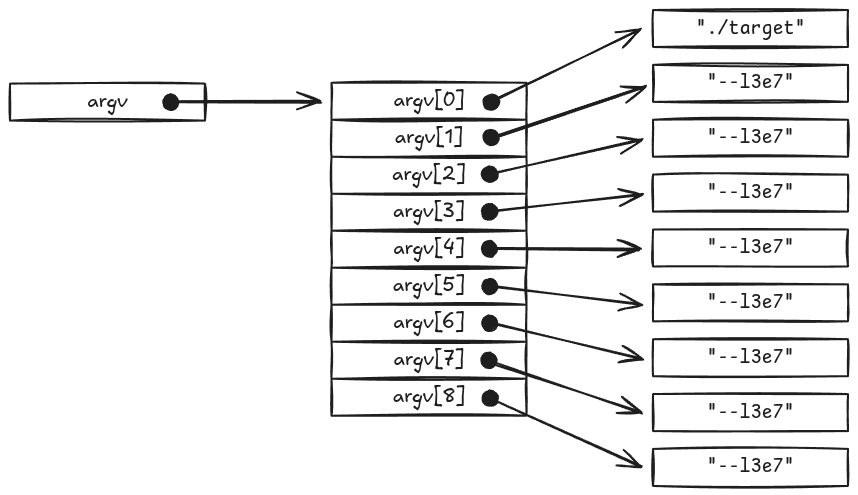
\includegraphics[width=\textwidth]{img/fsrv-prsvr-args.png}
         \caption{Reserve Space for argv Array} % 保留命令列參數陣列空間
         \label{fig:fsrv-prsvr-args}
     \end{subfigure}
     \begin{subfigure}[]{0.45\textwidth}
         \centering
         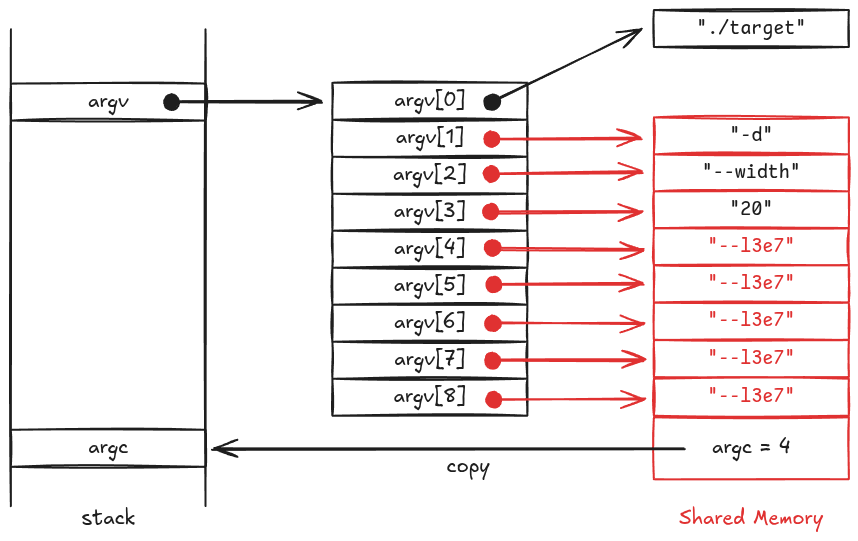
\includegraphics[width=\textwidth]{img/fsrv-chng-args.png}
         \caption{Shared Memory Sync} % 與共享記憶體同步
         \label{fig:fsrv-chng-args}
     \end{subfigure}
        \caption{Command-line Arguments Sync} % 命令列參數同步
        \label{fig:fsrv-sync-args}
\end{figure}

\fi % \subsection{Multi-Argument forkserver}